%%Berichtvorlage für EDBV WS 2015/2016

\documentclass[deutsch]{scrartcl}
\usepackage[ngerman]{babel}
\usepackage[utf8]{inputenc}
\usepackage{algorithmic}
\usepackage{algorithm}
\usepackage{graphicx}
\usepackage{amsmath,amssymb}
\usepackage{subcaption}
\captionsetup{compatibility=false}
\usepackage{multirow}
\usepackage{color}

\begin{document}

\title{Konzept: Verarbeitung von Grundrissen} %%Projekttitel hier eintragen

\subtitle{EDBV WS 2019/2020: AG\_E5} %%statt XX Arbeitsgruppenbezeichnung hier eintragen (zB.: A1)


%%Namen und Matrikelnummern der Gruppenmitglieder hier eintragen
\author{Leonhard Eder (00047514)\\
Raphael Schimmerl (00371366)\\
Florian Langeder (01527111)\\
Filip Hörtner (11808203)\\
Mark Alam (11808580)}

%%------------------------------------------------------

\maketitle


%%------------------------------------------------------

\section{Ziel}
Ziel des Projekts ist es, bestimmte Merkmale wie Wände, Türen, Fenster, Stiegen und Räume aus einem Grundrissplan zu erkennen und diese in einem Datensatz abzuspeichern.
%\textit{Kommentar: erklärt euer Projekt in einem Satz}
\section{Eingabe}
Als Eingabe verwenden wir 2D-Grundrisspläne in MATLAB-kompatiblen Datentypen. Unser Projekt wird auf dem Dataset \textit{cubicasa5k} (https://github.com/CubiCasa/CubiCasa5k) aufbauen, es können jedoch auch andere Grundrisse, die der in unseren Daten verwendeten Symbolik folgen, verarbeitet werden.
%\textit{Kommentar: Welche Eingabe benötigt euer Programm, muss der User Parameter wählen, etc. ?}
\section{Ausgabe}
Die Ausgabe ist eine Datei im JSON-Format, die die Auswertung der Analyse der Eingabedateien enthält. Enthalten sind: Anzahl der Räume, Fenster und Türen, Vorhandensein von Stiegen und die Größe der Räume (bei vorhandener Flächenangabe, sonst prozentuell).
%\textit{Kommentar: In welcher Form wird dem User der Output eures Programms präsentiert?}
\section{Voraussetzungen und Bedingungen}
Der Input besteht aus einem oder mehreren Graustufenbildern, die jeweils den Grundrissplan einer eingeschoßigen Wohnung darstellen. Die Notation der Symbole sollte der gängigen Symbolik entsprechen.

%\textit{Kommentar: Welche Eigenschaften muss der Input erfüllen, damit ihr damit arbeiten könnt (zB.: Kameraeinstellungen, Hintergrundeigenschaften, etc.)?}
\section{Methodik}
Methodik-Pipeline
\begin{enumerate}
	\item Umwandlung in ein Binärbild - Threshold nach Otsu
	\item Entfernung von Details - Kantenfilter
	\item Flächenbestimmung - Distanztransformation
	\item Erkennung der Türen und Abtrennung der Räume - Hough-Transformation
	\item Erkennung der Fenster - Kantenfilter
	\item Erkennung der Stiegen - Kantenfilter
\end{enumerate}

%\textit{Kommentar: Die folgenden Fragen sollten hier bedacht und beantwortet werden: Welche Arbeitsschritte sind notwendig um für den gegebenen Input den entsprechenden Output zu berechnen? Wozu sind die jeweiligen Methoden notwendig}
\section{Evaluierung}
\begin{itemize}
	\item Stimmen die Anzahlen der Räume, Türen, etc. überein?
	\item Werden alle Merkmale erkannt?
	\item Stimmen die Proportionen der Räume?
	\item Sind die berechneten Größen korrekt?
	\item Bei wie vielen Datensätzen wurde ein korrektes Ergebnis erzielt?

\end{itemize}
%\textit{Kommentar: Eine qualitative Evaluierung basiert auf der subjektiven Wahrnehmung einer Person (Ist ein Ergebnis gut oder schlecht?). Ihr sollte hier aber vor allem auch eine quantitative Evaluierung durchführen, d.h. eine objektive Evaluierung durch Vergleich eurer (Zwischen-)Ergebnisse mit ground truth (ein klassisches Beispiel: Für wie viele der Test-Datensätze wurde für Aufgabe xy ein korrektes Ergebnis erzielt?).}
\section{Datenbeispiel}
\begin{figure}[h!]
 \centering
 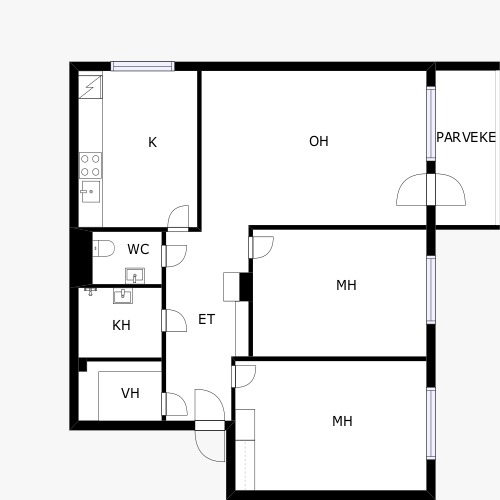
\includegraphics[width=0.4\textwidth]{model.png}
 \caption{Beispiel eines Grundrisses}
 \label{fig:img}
\end{figure}
\section{Zeitplan}
\begin{table}[h!]
	\centering
		\begin{tabular}{|c|c|c|}
		\hline
		Meilenstein & abgeschlossen am & Arbeitsaufwand in h\\
		\hline
		Erster Prototyp & 1.Dezember & 100h\\
		Anzahl der Räume & 20.Dezember & 25h\\
		Anzahl der Fenster & 20.Dezember & 25h\\
		Anzahl der Türen & 20.Dezember & 25h\\
		Stiegenerkennung & 20.Dezember & 25h\\
		Raumgrößen & 20.Dezember & 25h\\
		Tests, Evaluierung & 30.Dezember & 55h\\
		Bericht & 3.Jänner & 20h\\
		\hline
		\end{tabular}
\end{table}
%\textit{Kommentar: Definiert euch „Meilensteine“. Die vorgegebenen Termine (zB. Zwischenpräsentation) sind hier nicht von Interesse, stellt euch eher die Frage: Wann rechnet ihr mit einem fertigen Prototyp (mit Hilfe von Matlab-Toolboxes)? Wann soll danach ein gewisser Arbeitsschritt (entsprechend eurer Methodik-Pipeline) fertig implementiert sein? Plant auch Zeit für zB. Tests, Evaluierung etc. ein.
%Gebt weiters pro Arbeitsschritt an, wieviel Arbeitsaufwand (Stunden) eurer Meinung nach zur Umsetzung notwendig sind. Bedenkt, dass es sich bei EDBV um eine Übung im Ausmaß von 3.0 ECTs handelt. Für 1.0 ECTs rechnet man mit 25h Arbeitsaufwand pro Semester. Auf Teil1 (die Gruppenphase von EDBV) entfallen 2.4 dieser 3.0 ECTs und somit 60h Arbeit pro Gruppenmitglied. Wir rechnen daher für Teil 1 mit 300h Arbeit pro Gruppe.
%}
\begin{itemize}
	\item Stiegenerkennung: Leonhard Eder \cite{Dosch2000}
	\item Anzahl der Türen: Filip Hörtner \cite{TUW-274401}
	\item Größe der Räume: Raphael Schimmerl \cite{jang18}
	\item Anzahl der Fenster: Florian Langeder \cite{or2005highly}
	\item Anzahl der Räume: Mark Alam \cite{vargas18}
	
\end{itemize}
%\textit{Kommentar: Gebt eine relevante Literaturquelle (Bücher bzw. Kapitel, Konferenz- oder Journal-Papers) pro Gruppenmitglied (im kompilierten Bibtex-Format - Beispiele für Referenzen im Bibtex-Format: http://verbosus.com/bibtex-style-examples.html?lang=de). Diese Quellen sollten für euch bei zB. der Implementierung einer Methode, der Wahl von Parametern, etc. helfen. Können aber auch ein ähnliches Problem behandeln und motivieren, warum ihr euch für gewisse Methodik entschieden habt.}
%%------------------------------------------------------
\bibliographystyle{plain}
%\nocite{*}
\bibliography{edbv_lit}
%%Bei verwendung von Latex schreibt ihr eure Referenzen in ein eigenes bib-File (siehe hier Beispiel in edbv_lit.bib). Weitere Information zum Einbinden von BibTex gibt es hier: http://www.bibtex.org/Using/de/
%%------------------------------------------------------

\end{document}
